\documentclass{article}

\usepackage{tikz,tikz-qtree}

\begin{document}

\begin{center}
\begin{tikzpicture}
\Tree [.$A$ \texttt{a} [.$A$ \texttt{a} [.$A$ \texttt{a} [.$A$ \texttt{a} [.$A$ \texttt{a} [.$A$ \texttt{a} [.$B$ \texttt{b} [.$C$ [.$B$ \texttt{b} [.$C$ [.$B$ \texttt{b} [.$C$ [.$B$ \texttt{b} [.$C$ [.$B$ \texttt{b} [.$C$ [.$B$ \texttt{b} [.$C$ \texttt{c} ] ] \texttt{c} ] ] \texttt{c} ] ] \texttt{c} ] ] \texttt{c} ] ] \texttt{c} ] ] ] ] ] ] ] ]
\end{tikzpicture}
\end{center}

\begin{center}
\begin{tikzpicture}
\Tree [ \edge[dashed]; [.$B$ \texttt{b} [.$C$ [.$B$ \texttt{b} [.\node(n2){$C$}; [.$B$ \texttt{b} [.\node(n1){$C$}; \texttt{c} ] ] \texttt{c} ] ] \texttt{c} ] ] ]
\node[right of=n1] (label1) {$n_1$}; \draw[->] (label1)--(n1);
\node[right of=n2] (label2) {$n_2$}; \draw[->] (label2)--(n2);
\end{tikzpicture}
\end{center}

\begin{center}
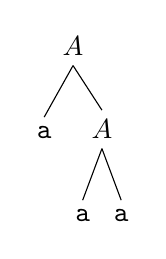
\begin{tikzpicture}
\Tree [.$A$ \texttt{a} [.$A$ \texttt{a} \texttt{a} ] ]
\end{tikzpicture}
\end{center}

\end{document}